\begin{table}[H]\centering\small
\begin{tabular}{lrrrr}\toprule
Method & Net utility & MC SE & Mean wealth & Mean max DD\\\midrule
Wait & 0.003655 & 0.000581 & 1.057 & 0.25\% \\
Economic quarter & 0.010747 & 0.000412 & 1.165 & 0.47\% \\
Hybrid & 0.013482 & 0.000805 & 1.217 & 0.63\% \\
Economic full & 0.042602 & 0.001652 & 1.875 & 1.88\% \\
\bottomrule\end{tabular}
\caption{Controlled exposure timing on all 100 fresh markets. Utility is mean
daily realized quadratic utility net of actual costs, multiplied by 252;
it is not annual return or certainty equivalent. Wealth starts at one and
compounds over 14 OOS years. DD denotes each path's maximum drawdown,
averaged across markets. All four methods retain noncrossings and losses.}
\label{tab:economic-authorization}
\end{table}
The primary paired Hybrid-minus-Wait utility difference is $0.009828$, with approximate pointwise 95\% Monte Carlo interval $[0.009219,0.010436]$. Hybrid-minus-Economic-full is $-0.029119$ with interval $[-0.030956,-0.027283]$; this secondary contrast is unadjusted. Evidence crosses at an annual review in 38 markets. 35 full-exposure authorizations are executed; 3 first crossings occur only at the terminal review. Intervals use the 100 paired markets and Student $t_{99}$, not daily observations.

All 100 markets initiate provisional exposure. In 0 markets the provisional period has negative cumulative realized utility, but the evaluator records 784 pre-deployment dates with negative conditional utility. These descriptive observations do not certify an absence of downside risk. All 1,400 annual target fits bind at the leverage cap; 0 markets change their target. Consequently the experiment identifies exposure timing for selected positions, without validating the uncertainty calibration or adaptive target sizing.

\begin{figure}[H]\centering
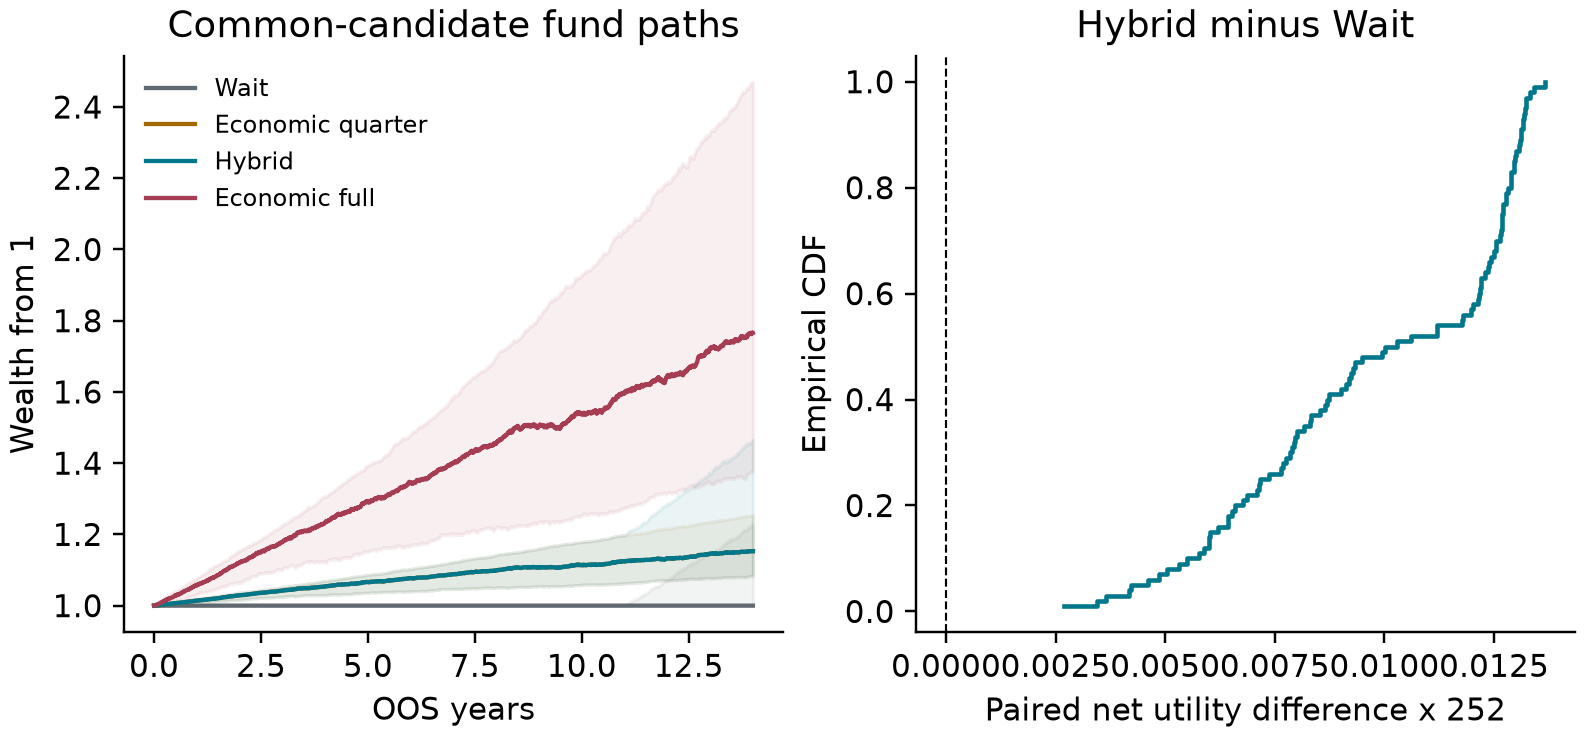
\includegraphics[width=\linewidth]{figures/economic_authorization.png}
\caption{All 100 new markets. Left: median wealth with 10th--90th market
quantiles, not confidence bands. Right: paired Hybrid-minus-Wait utility
differences. The candidate and fitting schedule are common; each fund pays
its own actual costs.}
\label{fig:economic-authorization}
\end{figure}
\FloatBarrier
